\section{Uvod}

Mobilni roboti, namenjeni za uporabo v nestrukturiranem naravnem okolju - gozdovi, gradbišča in področja naravnih nesreč, se pogosto poslužujejo uporabe koles v kombinaciji z kontroliranimi nogami, kjer žrtvujejo energijsko učinkovitost lažjemu prilagajanju terenu. Zadnje raziskave so prikazale, da se takšni kolesno-roboti lahko prilagajajo zahtevnemu okolju in imajo sposobnosti premagovanja ovir, vožnje po naklonini in zanesljivo delujejo v skrajnih okoljih, kot so gorske planote \cite{Wang2025Whee}.
  Krmilne strategije, ki poganjajo takšne robote so skoraj brez izjem učene s pomočjo spodbujevanega učenja (angl. RL, reinforcement learning), omogočeno s pomočjo GPU-po\-spe\-še\-nim izvajanjem več tisoč instanc fizikalnih simulacij na enkrat. V \cite{Rudin2022Lear} so pokazali, da lahko množično vzporedno učenje v kombinaciji z večfaznim učenjem na\-ra\-šča\-jo\-če težavnosti terena in motenj v nekaj minutah ustvari robustne politike hoje štirinožnih robotov ter da se politike, naučene izključno v simulaciji, brez dodatnega prilagajanja lahko neposredno prenesejo na fizično strojno opremo.
  
  Nadaljnje raziskave so se posvetile ugotovitvam, katere arhitekture so najboljše za uporabo kot strategijo v RL \cite{Smirnov2025RLBe}. Primerjali so usmerjene, povratne (LSTM, GRU), transformerske in arhitekture s prostorom stanj (Mamba) na podlagi različnih nalog krmiljenja z RL ter ugotovili, da so pri nalogah, ki zahtevajo vzpostavljanje ravnotežja in stabilnosti pod delnim opazovanjem stanj, pri omejeni strojni opremi najboljša izbira povratne arhitekture kot sta GRU (angl. gated recurrent unit) in LSTM (angl. long short term memory).

  V sorodnem delu \cite{Tofant2025Dife} so zasnovali agilnega dvokolesnega robota z zaprto kinematično verigo petih členov, pri čemer nogi vsake strani poganjata dva motorja in kolesi neposredno gnana motorja. Stabilizacijo nagiba robota so dosegli s kaskadnim regulatorjem sestavljenim iz notranje zanke, ki uporablja kvadratični integralni regulator (LQI) in zunanje zanke, poslužejoče se PID. Pristop eksplicitno ne uporablja globokega učenja pri čemer robot v vseh manevrih ravnotežje ohranja na obeh kolesih hkrati.
  
  V tem delu za dvokolesnega robota iz \cite{Tofant2025Dife} uvedemo krmilno strategijo, ki vzdržuje trajno, statično pozo na enem samem kolesu, stanje bistveno zahtevnejše od dvokolesnega ravnotežja. S tem, kolikor nam je znano, predstavljamo prvo naučeno strategijo za ohranjanje ravnotežja dvokolesnega robota na enem kolesu.
  
  Za reševanje obravnavane naloge ravnotežja smo predhodno preizkusili standardno usmerjeno nevronsko mrežo (angl. MLP, multilayer perceptron), vendar se je ta v prisotnosti senzornega šuma in časovnih zakasnitev izkazala za nestabilno ter ni konvergirala k zanesljivemu ravnotežju. Ti rezultati se skladajo z ugotovitvami študije \cite{Smirnov2025RLBe}, kjer avtorji ugotavljajo, da MLP mreže sicer omogočajo visoko učinkovitost, v okoljih z delno opazljivostjo pa odpovedo, zato smo kot osnovo strategije uporabili arhitekturo GRU z nevronsko mre\-žo, ki ji ni treba poznati niti eksplicitnega modela dinamike niti njegovih parametrov za posamezno konfiguracijo nog, s čimer nadaljujemo v smeri nadaljnjega dela, ki ga predlagajo avtorji \cite{Tofant2025Dife}.
  V nasprotju z GRU arhitekturami, primerjanimi v \cite{Smirnov2025RLBe} zgolj v simulacijskih okoljih, je naša povratna politika načrtovana in naučena za dejansko namestitev na vgrajenem mikrokrmilniku (STM32) pri nadzorni frekvenci 50 Hz, kar zahteva izjemno majhno strategijo za namen prenosljivosti strategije iz simulacijskega okolja v resnično, računsko omejeno strojno opremo za razliko od \cite{Rudin2022Lear}, kjer so uporabili bistveno zmogljivejši vgrajeni računalnik.
  
\begin{figure}[htbp] 
  \centering          
  \begin{tikzpicture}[scale=1]
    % Coordinates
    \coordinate (A) at (0.13, 0.14);
    \coordinate (B) at (-0.25, 0.25);
    \coordinate (C) at (0.75, -0.49);
    \coordinate (D) at (-0.75, 0.50);
    \coordinate (E) at (-1.00, 1.25);
    \coordinate (F) at (-0.30, -1.16);
    \coordinate (G) at (0.25, 1.25);
    \coordinate (H) at (1.00, 1.00);
    \coordinate (I) at (1.25, 1.25);
    \coordinate (J) at (1.00, 0.00);
    \coordinate (K) at (1.5, -0.25);
    \coordinate (L) at (-0.75, -1.00);
  
    % Drawing
    \node at (A.center) {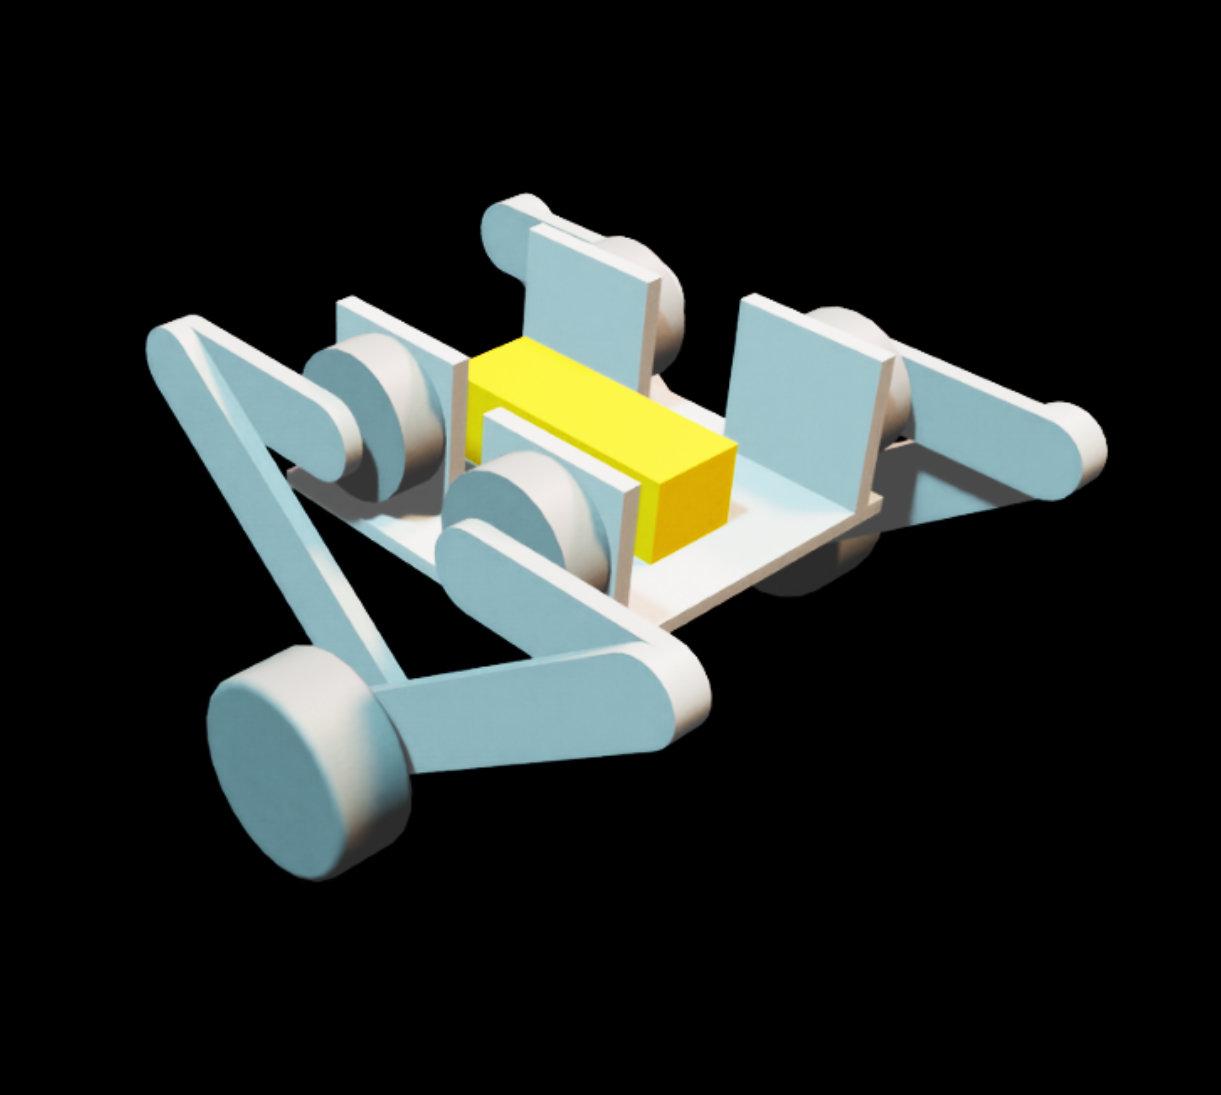
\includegraphics[width=4.00cm]{Images/Robot.png}};
    \draw[white] (B) -- (C);
    \draw[white] (D) -- (E);
    \node[below, text=white, font=\normalfont] at (F) {M3};
    \node[below, text=white, font=\normalfont] at (C) {M1};
    \node[above, text=white, font=\normalfont] at (E) {M2};
    \node[above, text=white, font=\normalfont] at (G) {M5};
    \node[above] at (H) {$x$};
    \node[above] at (H) {$x$};
    \draw[white] (H) -- (I);
    \node[above, text=white, font=\normalfont] at (I) {M4};
    \draw[white] (J) -- (K);
    \node[below, text=white, font=\normalfont] at (K) {M6};
    \draw[white] (L) -- (F);
  \end{tikzpicture}
\caption{USDC model robotske platforme z označenimi motorji M1--M6.}
\label{robot} 

\end{figure} 

%Kolesno-nožni roboti združujejo hitrost in agilnost z učin\-ko\-vi\-to\-stjo vožnje ter gibljivostjo nog, kar predstavlja že\-lje\-no kombinacijo sposobnosti robota v nestrokturiranih okoljih \cite{Liu2024Deve,Wang2025Whee}. Posebej zanimivi so dvokolesni roboti, ki delujejo po načelu inverznega nihala, zaradi česar pa so inherentno nestabilni. S tem se soočijo z enim izmed glavnih problemov sodobne mobilne robotike, v kateri je vedno popularnejša humanoidna robotika \cite{Bao2025Deep}. V članku \cite{Tofant2025Dife} so problem regulacije naklona dvokolesnega robota rešili s pomočjo notranje in zunanje zanke kaskadnega regulatorja, kjer notranja zanka uporablja kvadratični integralni regulator (angl. Linear Quadratic Integral controller, LQI), ki se je izkazal kot robustna rešitev vodenja robota v različnih okoljih. Razčlenitev njihovega regulatorja na dve regulaciji, za vsako kolo posebej, pa odpre vrzel v problemu, ki ga obravnavamo v tem delu; to je regulacija dvokolesnega robota, tako da stoji le na enem kolesu. Gre za nestabilen, sklopljen regulacijski problem: naklon je mogoče uravnavati le s pomočjo pogonskega kolesa, bočni nagib pa le s sklepi noge, pri čemer ravnovesna lega ni pokončna, temveč nagnjena.
  
  %Rešujemo  ga z globokim spodbujevalnim učenjem v simulaciji. Namesto da bi ravnovesni kot predpisali, funkcijo nagrajevanja zasnujemo tako, da ga politika med učenjem poišče sama; območje začetnih pogojev postopoma širimo s samodejnim kurikulumom, prenos iz simulacije na realni sistem pa dosežemo z randomizacijo domene, prilagojeno lastnostim dejanske strojne opreme. Rešitev je zasnovana tako, da se izvaja neposredno na vgrajenem mikrokrmilniku robota.
  %V našem primeru imamo tako zraven dinamike naklona še sklopljenost dinamike po nagibu, medtem ko imamo le eno stično točko, kar s klasičnim modelom \cite{Tofant2025Dife} težko opišemo, izpeljava analitičnega modela za tako lego pa je zahtevna. Avtorji v prispevku \cite{Tofant2025Dife} izrecno navajajo, da je uporaba strojnega učenja smiselna za nadaljnje delo. V našem primeru pa smo regulator nadgradili z uporabo pristopa spodbujevanega učenja (angl. reinforcement learning, RL), kjer se regulator uči na podlagi mnogih poskusov lovljenja ravnotežja v simulacijskem okolju, brez eksplicitno nastavljenega modela sklopljene dinamike \cite{Bao2025Deep}. Namesto da bi ravnovesni kot predpisali, funkcijo nagrajevanja zasnujemo tako, da ga politika med uče\-njem poišče sama, saj območje začetnih pogojev postopoma širimo z večfaznim učenjem. S tem se regulator nauči strategije (angl. policy), ki je robustna na celotno porazdelitev fizikalnih parametrov, upoštevajoč randomizacije domene (angl. domain randomization) prilagojeno lastnostim dejanske strojne opreme, kar omogoči uporabo strategije na realnem robotskem sistemu. 